% Standalone section build preserving the available article template.
% The full-paper master and its preceding equations were not supplied.
\documentclass[10pt]{article}
\usepackage[margin=22mm]{geometry}
\usepackage{amsmath,amssymb,graphicx,algorithm,algpseudocode}
\begin{document}
% Preview numbering: objective(3), problem(4), P1(5), P2(6), stopping(7).
% Do NOT copy this counter adjustment into the full paper: use its real counters.
\setcounter{equation}{2}
% Insert into the paper after its channel/security definitions. nu_MB is nu_raw.
\section{Joint Optimization of Modulation Variance and Maxwell--Boltzmann Shaping Parameter}
\label{sec:joint-modulation-optimization}

\subsection{SKR Performance Optimization}
Modulation variance $V_A$ and the Maxwell--Boltzmann (MB) shaping parameter
$\nu_{\rm MB}$ jointly determine the probabilities and physical amplitudes
of the 256 coherent states. Increasing variance changes both Bob's information
and Eve's Holevo information; changing shaping also changes the amplitude
normalization required at a given variance. Consequently, maximizing mutual
information alone, or optimizing either parameter at an arbitrary fixed value
of the other, does not generally maximize the numerical secret-key-rate (SKR)
objective. For each declared link distance $L$, we consider the maintained
asymptotic reverse-reconciliation calculation
\begin{equation}
 K(L,\nu_{\rm MB},V_A)=\beta_{\rm rec}I_{AB}(L,\nu_{\rm MB},V_A)
 -\chi_{BE}(L,\nu_{\rm MB},V_A;Z_-),\qquad \beta_{\rm rec}=0.95.
 \label{eq:joint-skr-objective}
\end{equation}
The deterministic discrete-input heterodyne MI and direct-$Z_-$ Holevo
calculation use the same normalized ensemble and excess noise. The existing
source-moment definitions, arbitrary-precision policy and quadrature are
unchanged. This section concerns the declared direct-$Z_-$ numerical experiment,
not full-$Z$-interval certification or an enlarged security claim.

\subsection{Joint Optimization Problem}
The intended MB-family problem is
\begin{equation}
 \mathcal P:\quad\max_{\nu_{\rm MB}\ge0,\,V_A>0}
 K(L,\nu_{\rm MB},V_A).
 \label{eq:joint-modulation-problem}
\end{equation}
Here $\nu_{\rm MB}$ denotes the stored raw square-QAM parameter
$\nu_{\rm raw}$, not the internally rescaled parameter
$\nu_{\rm repo}=42.5\nu_{\rm raw}$. All reported pairs use the raw convention.
This experiment imposes neither a peak-photon constraint nor a common energy
budget or preset upper bound on the optimization variables. Finite numerical
brackets are search devices, not additional physical constraints.

The implementation searches $\nu_{\rm MB}>0$, although the intended family
in Eq.~\eqref{eq:joint-modulation-problem} includes zero. At zero the MB PMF
reduces to Uniform. Compatible stored Uniform results independently sample
this endpoint under the same channel and security conventions, but do not
certify maximization over every $V_A>0$ on that boundary. Uniform is not an
AO start or a member of the positive-$\nu$ MB catalog. Thus, the reported AO
results retain this endpoint-coverage limitation rather than silently changing
the intended feasible domain.

\subsection{Alternating Optimization Algorithm}
For a start indexed from $r=0$, the maintained alternating optimization (AO)
updates are
\begin{align}
 \mathcal P_1:\quad V_A^{(r)}&\approx\underset{V_A>0}{\arg\max}
 K(L,\nu_{\rm MB}^{(r-1)},V_A),\label{eq:p1}\\
 \mathcal P_2:\quad \nu_{\rm MB}^{(r)}&\approx\underset{\nu_{\rm MB}>0}{\arg\max}
 K(L,\nu_{\rm MB},V_A^{(r)}).\label{eq:p2}
\end{align}
The approximation signs distinguish the actual finite coordinate searches from
exact continuous argmax operations. P1 holds the preceding shaping parameter
fixed; P2 holds the newly selected variance fixed. Algorithm~\ref{alg:ao}
records the implementation's updates and diagnostic stopping states.

Each coordinate search evaluates every compatible available point on its
fixed-coordinate slice. An endpoint winner triggers exact half-value or
double-value requests, with at most three expansion attempts. An interior
winner $z$, with nearest evaluated neighbors $z_-<z<z_+$, is refined through
the paired requests $(z_-+z)/2$ and $(z+z_+)/2$, in that order. The radius
$\max(z-z_-,z_+-z)$ is tested against $\epsilon_p=10^{-6}$ at loop entry.
At most four refinement stages are attempted; there is no additional tolerance
check after the fourth stage. A singleton or an exhausted expansion cap does
not close both outer directions. Missing source moments and numerical failures
remain explicit events; no moments or objective values are interpolated.

The initial raw shaping parameters are $0.1$, $0.15$, $0.3$, and $0.8$.
Each start uses an available supplied variance or, otherwise, the smallest
available positive variance on its slice. After the first distance, the
preceding selected pair is appended as a warm start. The valid terminal result
with largest recorded SKR is selected in the original start order for ties,
and independently compared with the maximum of the compatible finite catalog.
This does not imply that every individual start attains that maximum.

% Same implementation as the previous Algorithm 1; notation aligned with P1/P2.
\begin{algorithm}[t]
\caption{Exact-source alternating optimization with explicit search status}
\label{alg:ao}
\small
\begin{algorithmic}[1]
\Require Frozen channel and distance $L$; compatible caches; optional previous-distance pair;
$R_{\max}=6$, $\epsilon=10^{-8}$, $\epsilon_p=10^{-6}$, $J=4$, $B=3$
\Ensure Best recorded terminal pair/SKR and diagnostic status
\State Form starts $\nu_0\in\{0.1,0.15,0.3,0.8\}$; append the previous-distance pair if available
\For{each start in the original order}
 \State Choose an available supplied $V_{A,0}$ or the smallest available positive slice value
 \State Initialize $x^{(0)}=(\nu_0,V_{A,0})$, $K^{(0)}=K(L,x^{(0)})$; record failure and skip invalid initialization
 \State $u\gets\mathrm{false}$; $s\gets\texttt{MAX\_ITERATIONS\_REACHED}$
 \For{$r=1,\ldots,R_{\max}$}
  \State Snapshot the last complete $x^{(r-1)}=(\nu_{\rm MB}^{(r-1)},V_A^{(r-1)})$ and $K^{(r-1)}$
  \State $q_1\gets\Call{CoordinateSearch}{V_A,\nu_{\rm MB}^{(r-1)},\epsilon,\epsilon_p,J,B}$
  \State If $q_1$ has no valid best point, record its failure status and stop this start
  \State $\widetilde V_A\gets q_1.\mathrm{best}.V_A$ \Comment{P1, Eq.~\eqref{eq:p1}}
  \State $q_2\gets\Call{CoordinateSearch}{\nu_{\rm MB},\widetilde V_A,\epsilon,\epsilon_p,J,B}$
  \State If $q_2$ has no valid best point, record its failure status and stop this start
  \State Commit $x^{(r)}=(q_2.\mathrm{best}.\nu_{\rm MB},\widetilde V_A)$ and $K^{(r)}=q_2.\mathrm{best}.K$
  \State Record both phase updates and coordinate statuses
  \State $u\gets u\lor\neg(\Call{Closed}{q_1}\land\Call{Closed}{q_2})$
  \State $\delta K\gets K^{(r)}-K^{(r-1)}$
  \If{nonfinite $\delta K$, $\delta K<-\epsilon$, a monotonicity warning or recorded numerical failures}
   \State $s\gets\texttt{NUMERICAL\_FAILURE}$; \textbf{break}
  \ElsIf{$|\delta K|\le\epsilon$} \Comment{Eq.~\eqref{eq:ao-stopping}}
   \If{either coordinate has an unclosed boundary}
    \State $s\gets\texttt{UNRESOLVED\_BOUNDARY}$
   \ElsIf{$u$ or either coordinate is incomplete}
    \State $s\gets\texttt{STAGNATED\_IN\_EXACT\_CATALOG}$
   \Else
    \State $s\gets\texttt{CONVERGED\_NUMERICALLY}$
   \EndIf
   \State \textbf{break}
  \EndIf
 \EndFor
 \State Retain the last complete P1--P2 update and status $s$
\EndFor
\State Select the valid terminal result with largest recorded $K$; retain original order for ties
\State Independently compare with the compatible catalog maximum and report unresolved scope
\end{algorithmic}
\end{algorithm}


\subsection{Stopping Criteria and Parameter Selection}
With $K^{(r)}=K(L,\nu_{\rm MB}^{(r)},V_A^{(r)})$, the original objective-change
condition is
\begin{equation}
 \left|K^{(r)}-K^{(r-1)}\right|\le\epsilon,
 \qquad \epsilon=10^{-8}\ \mathrm{bits/use}.
 \label{eq:ao-stopping}
\end{equation}
The outer cap $R_{\max}=6$ bounds complete AO cycles, whereas $\epsilon$
detects small SKR changes. Neither alone establishes optimality. When the
condition holds, the code reports an unresolved boundary if present,
otherwise catalog stagnation if either coordinate is incomplete or an
earlier search in the same start was unresolved. A numerical-convergence
status requires both coordinates to be closed, no missing moments or
numerical failures, and no earlier unresolved search. Monotonicity and
numerical-failure checks precede the objective-change decision.

We examined the sixteen combinations of $R_{\max}\in\{4,6,8,10\}$ and
$\epsilon\in\{10^{-6},10^{-7},10^{-8},10^{-9}\}$ using the same 147 exact
source pairs and 26 distances. All other settings and search logic were
fixed; each configuration used all original starts and its own ordered
previous-distance warm-start chain. The baseline first reproduced all 129
recorded starts, 283 outer updates, histories and terminal states. The
objective tolerance also retains its original role in endpoint-improvement
and monotonicity checks; the parameter-radius tolerance remains $10^{-6}$.

Every setting selected identical parameter pairs and SKR values at all 26
distances, with zero deviation from the baseline finite-catalog maxima.
Increasing the cap to eight or ten produced no improvement; four also
reproduced the catalog result. All starts stopped by the fourth cycle, and
none terminated because of the cap itself. Thus, six is a conservative
computational safeguard for these evaluated cases, not a theoretically
optimal count or a guarantee of convergence.

Tightening $\epsilon$ from $10^{-8}$ to $10^{-9}$ changed neither solutions
nor the 283-cycle total. Loosening it to $10^{-6}$ reduced this total to 279
without changing any selected or individual terminal solution: four starts
at $22$ km stopped one cycle earlier, with a positive increment of
$5.488961496435962\times10^{-7}$ bits/use. Table~\ref{tab:ao-stopping-sensitivity}
groups the identical outcomes across caps; Table~\ref{tab:ao-stopping-detail}
retains all sixteen settings. Figures~\ref{fig:rmax-sensitivity} and
\ref{fig:epsilon-sensitivity} show the actual tested reference and $22$ km
values, without fitting or interpolating additional settings.

\begin{table}[t]
 \centering\small
 \caption{Stopping sensitivity over 26 distances. Each row represents four
 separate configurations, $R_{\max}\in\{4,6,8,10\}$; entries apply to each
 configuration, not their sum. Same denotes identical selected binary64 pairs;
 $N_{\rm cyc}$ is the aggregate count over 129 starts. Closed counts include
 52 selected-final postchecks per configuration.}
 \label{tab:ao-stopping-sensitivity}
 \begin{tabular}{rrrrr}
 \hline
 $\epsilon$ & Same & $\max|\Delta K|$ & $N_{\rm cyc}$ & Closed \\
 \hline
 $10^{-6}$ & 26/26 & 0 & 279 & 0/610 \\
 $10^{-7}$ & 26/26 & 0 & 283 & 0/618 \\
 $10^{-8}$ & 26/26 & 0 & 283 & 0/618 \\
 $10^{-9}$ & 26/26 & 0 & 283 & 0/618 \\
 \hline
 \end{tabular}
\end{table}


Each configuration retained 20 catalog-stagnation and 109 unresolved-boundary
terminal states, and all 129 starts requested missing source moments. No
coordinate search completed. Zero-increment incomplete termination occurred
in 129 starts for $\epsilon\le10^{-7}$ and 125 for $\epsilon=10^{-6}$.
Consequently, the observed insensitivity is conditional on incomplete
exact-source coverage. Inner searches reconstruct brackets from available
points rather than carrying pending refinement across cycles; an unchanged
cached winner can trigger stopping before a larger outer cap is reached.
The total SKR numerical error has not been bounded. The baseline
$\epsilon=10^{-8}$ is therefore an objective-stagnation threshold, not a
certified absolute accuracy. Neither its superiority to $10^{-6}$ nor
continuous convergence is demonstrated by this experiment.

\begin{figure}[t]
 \centering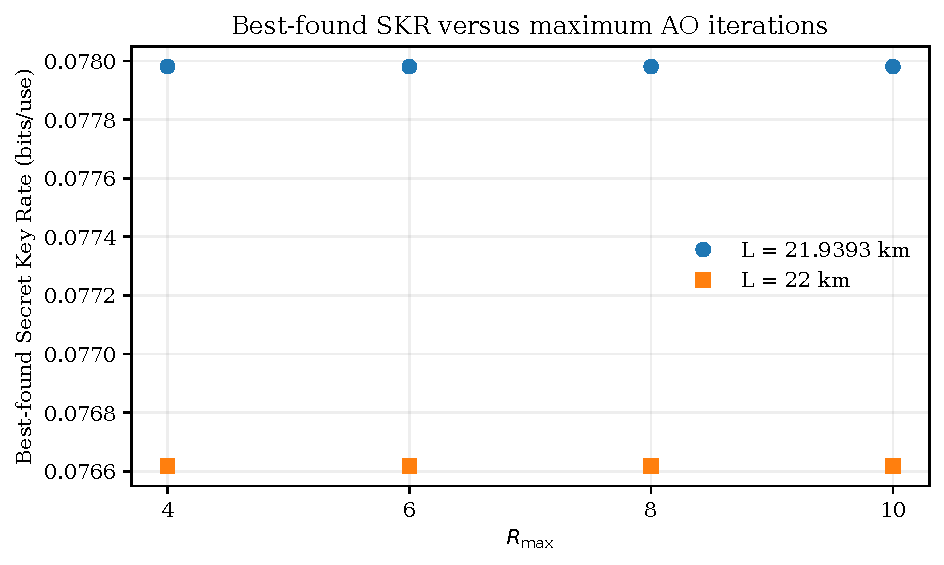
\includegraphics[width=\linewidth]{figures/rmax_sensitivity.pdf}
 \caption{Best-found SKR at the tested caps, with $\epsilon=10^{-8}$.
 Each marker is an actual cache-only AO result. Identical values do not
 imply completed coordinate searches.}
 \label{fig:rmax-sensitivity}
\end{figure}
\begin{figure}[t]
 \centering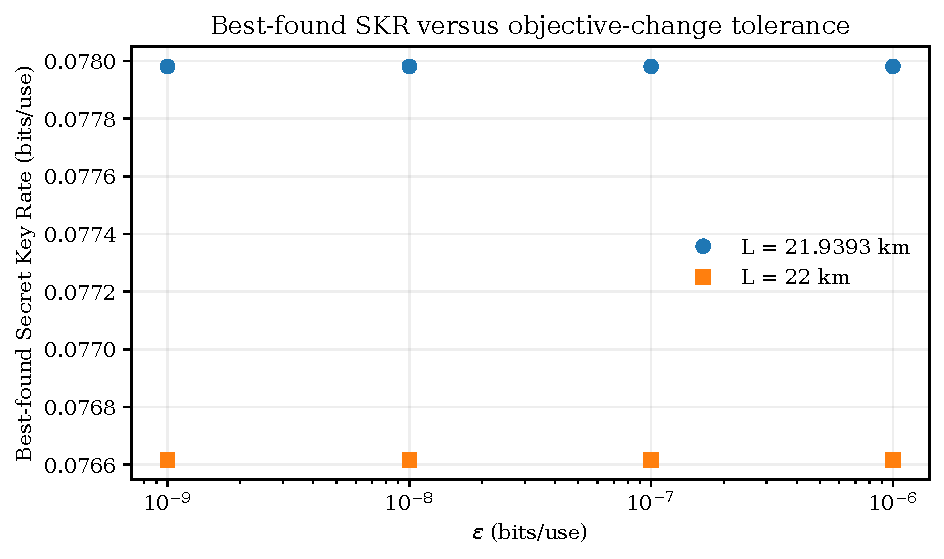
\includegraphics[width=\linewidth]{figures/epsilon_sensitivity.pdf}
 \caption{Best-found SKR at the tested objective-change thresholds, with
 $R_{\max}=6$ and a base-10 logarithmic tolerance axis. The selected SKR
 remains unchanged; the aggregate iteration count decreases at $10^{-6}$.}
 \label{fig:epsilon-sensitivity}
\end{figure}


\subsection{Numerical Optimization Results}
The compatible catalog contains 147 distinct MB source pairs and 3,822 stored
objective values over 26 link distances. Baseline AO records comprise 129
starts and 283 complete outer updates. At each distance, the best selected
terminal result matches the independently ranked maximum of the 147 stored
values. Only 59 of the 129 individual terminal results attain their distance's
catalog maximum; no distance exhibits unanimous agreement across its starts.
We therefore report best-found numerical solutions and finite-catalog maxima,
not certified continuous-domain optima.

At the reference distance $L=21.9393102292$ km, the selected raw pair is
$(\nu_{\rm MB},V_A)=(0.165,5.5)$, with
\begin{align*}
 I_{AB}&=0.6341892631163653, & \beta_{\rm rec}I_{AB}&=0.602479799960547,\\
 \chi_{BE}&=0.5244988060866094, & K_{\rm best}&=0.07798099387393764\ \mathrm{bits/use}.
\end{align*}
At $22$ km, the selected pair is $(0.165,5.475)$ with
$K_{\rm best}=0.07661740491526092$ bits/use. These decimal representations
reproduce the stored numerical values; their printed precision is not an
absolute-error guarantee. The complete 26-distance parameters are summarized
in Table~\ref{tab:ao-parameters-26}; the supplied CSV retains full stored precision.

Figures~\ref{fig:ao-history} and \ref{fig:ao-parameters} show genuine recorded
updates. At the reference distance four of five starts attain the selected
pair. The $\nu_0=0.8$ start instead follows
$(0.8,1.5)\to(0.5,1.5)\to(0.4,3.0)\to(0.4,3.0)$ and ends at
$K=0.06912585821984563$ bits/use. Its final coordinate requests lack moments
at $(0.4,1.5)$ and $(0.2,3.0)$. The lower terminal value is therefore not
evidence of a distinct converged basin.

\begin{figure}[t]
 \centering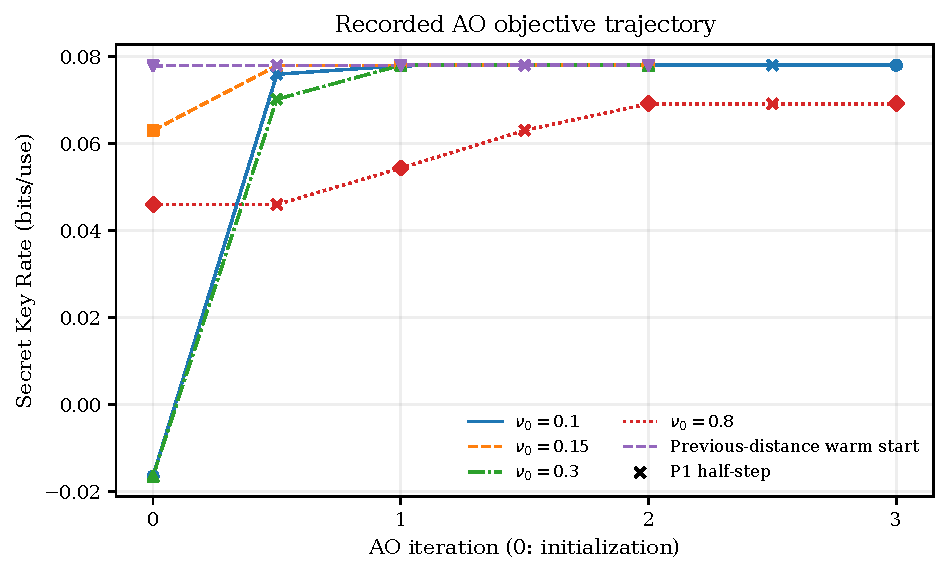
\includegraphics[width=\linewidth]{figures/ao_convergence.pdf}
 \caption{Genuine AO objective histories at the reference distance. Crosses
 denote P1 half-steps and integer markers denote complete P1--P2 cycles.
 Flat portions with incomplete searches are not convergence certificates.}
 \label{fig:ao-history}
\end{figure}
\begin{figure}[t]
 \centering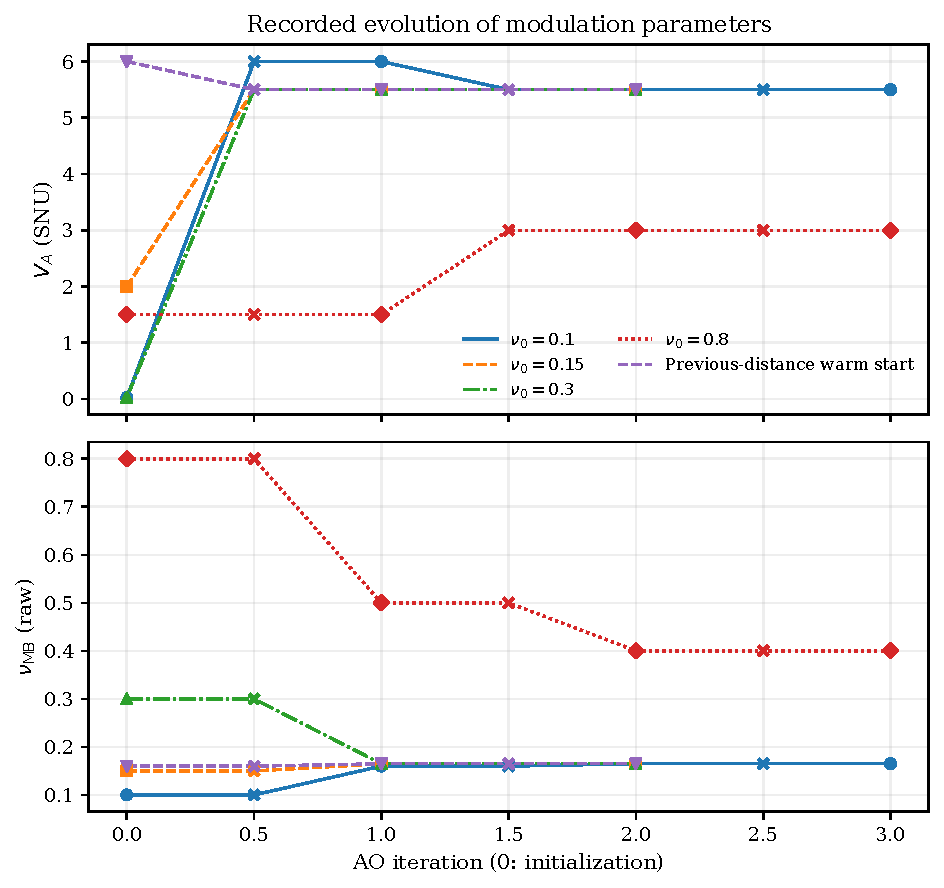
\includegraphics[width=\linewidth]{figures/ao_parameter_evolution.pdf}
 \caption{Recorded variance and raw shaping-parameter updates for the same
 starts. Connecting lines guide the eye between recorded events; they are
 not interpolated evaluations.}
 \label{fig:ao-parameters}
\end{figure}

Figure~\ref{fig:skr-distance} compares the stored Uniform results, the fixed
MB reference and the AO-selected MB curve on the established grid. The
full-angle divergence is $10~\mu\mathrm{rad}$, receiver diameter $0.55$ m,
beam waist $0.0986760647169751$ m, HAP/UAV altitudes $20/1$ km, wavelength
$1550$ nm and zenith atmospheric transmittance $0.92$. Optical adaptive
optics and phase noise are off; channel excess noise is $0.0186$ SNU.
Optical adaptive optics is distinct from the AO optimization algorithm.
The fixed MB pair is $(0.2,1.3833230302980657)$ at every distance.
The AO-selected result exceeds that reference at all 26 evaluated distances.
At the reference distance, fixed MB gives $0.05268768994955189$ bits/use;
at $40$ km the selected pair $(0.15,3.5548673904962893)$ gives
$0.00225888275226813$ bits/use, versus $0.0016507968216343365$ for fixed MB.
These are stored-sample, unconstrained-modulation comparisons, not range
extrapolations or energy-constrained hardware-throughput claims.

\begin{figure}[t]
 \centering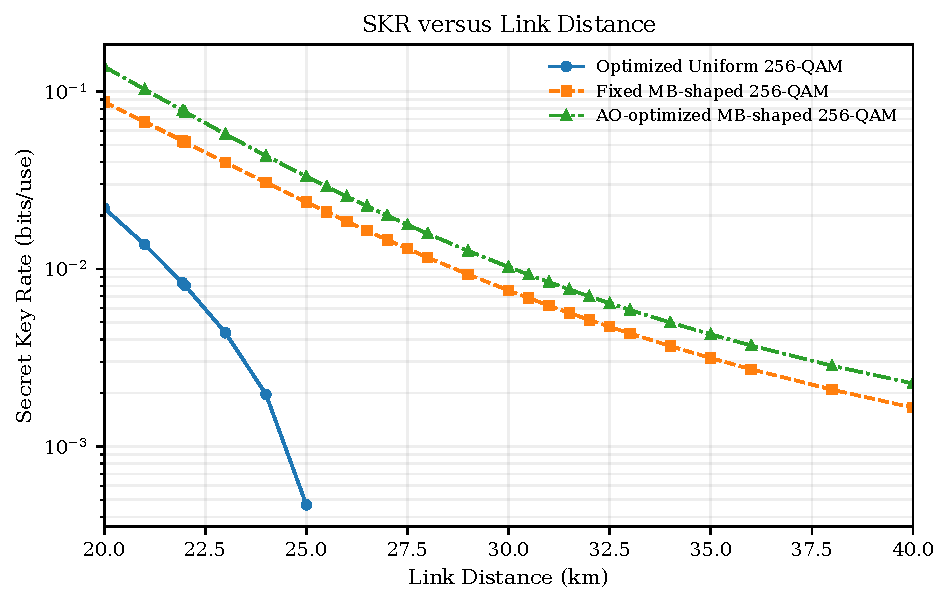
\includegraphics[width=\linewidth]{figures/skr_vs_distance.pdf}
 \caption{Compatible stored SKR results versus link distance. AO-optimized
 MB denotes the selected finite-catalog result. The Uniform curve represents
 its historical best-tested search, not a certified continuous optimum.
 Only positive exact samples are shown on the base-10 logarithmic axis:
 Uniform ends at $25$ km and both MB curves reach $40$ km. Non-positive values
 remain unchanged in the original data; no zero crossing is interpolated.}
 \label{fig:skr-distance}
\end{figure}

\subsection{Numerical Limitations}
All baseline starts contain incomplete coordinate searches: 20 terminate as
\texttt{STAGNATED\_IN\_EXACT\_CATALOG} and 109 as
\texttt{UNRESOLVED\_BOUNDARY}. Across the sensitivity experiments, zero of
9,856 coordinate calls complete; this count includes 832 selected-final
postchecks in addition to 9,024 calls within the 4,512 outer updates. The 55
distinct missing source pairs are the union of requests over the distances
and settings, not 55 newly executed calculations.

At the reference selected pair, P1 remains bracketed by $[5.4875,5.5125]$
and requests $(0.165,5.49375)$ and $(0.165,5.50625)$. P2 at $V_A=5.5$
has bracket $[0.1625,0.16562500000000002]$ and requests $(0.16375,5.5)$
and $(0.16531250000000003,5.5)$. Keeping the incumbent fixed would require
14 and 12 midpoint-halving levels, respectively, to reduce the present radii
to $10^{-6}$. These are conditional geometric estimates, not performed
refinement steps or convergence guarantees. The $22$ km shaping slice at
$V_A=5.475$ has only one compatible exact point and is not closed.

The inner cap, repeated reconstruction of brackets, missing moments, persistent
unresolved flag, unclosed outer directions, Uniform-endpoint coverage and
unbounded total SKR numerical error prevent certification of coordinate-wise
continuous convergence or a global optimum. The supported contribution here
is reproducible joint best-found performance and independently checked
finite-catalog maximization with transparent numerical limitations. No
finite-size, composable-security or publication-scale lifecycle certification
is inferred from this manuscript preparation.

\clearpage
\appendix
\section{Detailed Stopping-Parameter Sensitivity}
\begin{table}[htbp]
\centering\small
\caption{All sixteen settings. $N_{\rm cyc}$ counts outer updates over129 starts; closed includes52 final postchecks. Every row has129 missing-source-blocked starts,20 catalog-stagnation and109 unresolved-boundary states.}
\label{tab:ao-stopping-detail}
\begin{tabular}{rrrrrr}
\hline
$R_{\max}$ & $\epsilon$ & Same & $\max|\Delta K|$ & $N_{\rm cyc}$ & Closed \\
\hline
4 & $10^{-6}$ &26/26 &0 &279 &0/610 \\
4 & $10^{-7}$ &26/26 &0 &283 &0/618 \\
4 & $10^{-8}$ &26/26 &0 &283 &0/618 \\
4 & $10^{-9}$ &26/26 &0 &283 &0/618 \\
6 & $10^{-6}$ &26/26 &0 &279 &0/610 \\
6 & $10^{-7}$ &26/26 &0 &283 &0/618 \\
6 & $10^{-8}$ &26/26 &0 &283 &0/618 \\
6 & $10^{-9}$ &26/26 &0 &283 &0/618 \\
8 & $10^{-6}$ &26/26 &0 &279 &0/610 \\
8 & $10^{-7}$ &26/26 &0 &283 &0/618 \\
8 & $10^{-8}$ &26/26 &0 &283 &0/618 \\
8 & $10^{-9}$ &26/26 &0 &283 &0/618 \\
10 & $10^{-6}$ &26/26 &0 &279 &0/610 \\
10 & $10^{-7}$ &26/26 &0 &283 &0/618 \\
10 & $10^{-8}$ &26/26 &0 &283 &0/618 \\
10 & $10^{-9}$ &26/26 &0 &283 &0/618 \\
\hline
\end{tabular}
\end{table}

\section{Best-Found Parameters on the Established Distance Grid}
\begin{table}[htbp]
\centering\small
\caption{Selected finite-catalog maxima. Parameters use raw MB convention. Values are rounded for presentation only; the supplied CSV preserves exact stored binary64 values.}
\label{tab:ao-parameters-26}
\begin{tabular}{rrrr}
\hline
$L$ (km) & $\nu_{\rm raw}$ & $V_A$ (SNU) & $K$ (bits/use) \\
\hline
20.0 &0.15 &6.5 &0.1380135313 \\
21.0 &0.16 &6 &0.1027071638 \\
21.9393102292 &0.165 &5.5 &0.07798099387 \\
22.0 &0.165 &5.475 &0.07661740492 \\
23.0 &0.165 &5.3 &0.05745739941 \\
24.0 &0.15 &5 &0.04337158783 \\
25.0 &0.15 &4.5 &0.03315573558 \\
25.5 &0.15 &4.5 &0.02909451458 \\
26.0 &0.15 &4.5 &0.0255988033 \\
26.5 &0.15 &4.5 &0.02258632179 \\
27.0 &0.15 &4.5 &0.01998644158 \\
27.5 &0.15 &4.5 &0.0177387778 \\
28.0 &0.15 &4.5 &0.01579185679 \\
29.0 &0.15 &3.5548673905 &0.01263375261 \\
30.0 &0.15 &3.5548673905 &0.010253504 \\
30.5 &0.15 &3.5548673905 &0.009278128392 \\
31.0 &0.15 &3.5548673905 &0.008419975631 \\
31.5 &0.15 &3.5548673905 &0.007663135178 \\
32.0 &0.15 &3.5548673905 &0.006994021456 \\
32.5 &0.15 &3.5548673905 &0.006401020851 \\
33.0 &0.15 &3.5548673905 &0.005874192306 \\
34.0 &0.15 &3.5548673905 &0.004986168364 \\
35.0 &0.15 &3.5548673905 &0.004275173307 \\
36.0 &0.15 &3.5548673905 &0.00370055444 \\
38.0 &0.15 &3.5548673905 &0.002846344525 \\
40.0 &0.15 &3.5548673905 &0.002258882752 \\
\hline
\end{tabular}
\end{table}

\end{document}
